\chapter{Algoritmi utilizzati} %\label{1cap:spinta_laterale}
% [titolo ridotto se non ci dovesse stare] {titolo completo}
%
\begin{citazione}
Nell'ambito del presente capitolo sarà effettuata una trattazione degli algoritmi utilizzati dalla \emph{pipeline} che si intende implementare. La trattazione in questione è volta all'analisi delle motivazioni che hanno portato alla scelta degli algoritmi stessi. Verranno, in primo luogo, descritti nel dettaglio gli algoritmi di base che sono stati scelti per costruire la \emph{pipeline}; successivamente verranno passate a rassegna le modifiche apportate a tali algoritmi al fine di aggiungere un layer di sicurezza alla \emph{pipeline}. 
\end{citazione}
\newpage

\section{Pipeline iniziale}
Gli autori di \cite{zeng2018secure} hanno proposto una \emph{pipeline} composta da diversi algoritmi, alcuni dei quali opportunamente modificati al fine di aggiungere un layer di sicurezza al processo di compressione. Nelle sezioni successive verrà fornita una descrizione delle versioni di base di tali algoritmi volta all'agevolazione della comprensione del funzionamento dell'algoritmo complessivo. L'algoritmo di compressione \emph{lossless} di partenza prenderà in input un testo $T$ da comprimere e sarà composto da \emph{Burrows-Wheeler Transform, Move-To-Front, Run-Length Encoding e Variable Length Prefix Code}, restituendo un testo compresso $C$. Specularmente, l'algoritmo di decompressione prenderà in input il testo compresso $C$ e sarà composto da \emph{Inverse Variable Length Prefix Code, Inverse Run-Length Encoding, Inverse Move-To-Front e Inverse Burrows-Wheeler Transform}, restituendo il testo non compresso di partenza $T$.
\subsection{Burrows-Wheeler Transform} 
La \textbf{Burrows-Wheeler Transform (BWT)} è un algoritmo utilizzato in diversi programmi di compressione come \emph{bzip}, tuttavia è importante precisare che non si tratta di un algoritmo di compressione in quanto ha come unico scopo quello di permutare l'ordine dei caratteri della stringa input. Il funzionamento della \emph{BWT} si suddivide in tre step fondamentali:
\begin{enumerate}
    \item Data una stringa input $S$ definita su un alfabeto $\Sigma$, si aggiunge un carattere speciale $\$ \notin \Sigma$ alla fine della stringa $S$ ottenendo la stringa $S'$. Il carattere $\$$ sarà più piccolo in ordine lessicografico rispetto ad ogni altro carattere di $\Sigma$;
    \item Si costruisce una matrice $M$ le cui righe sono gli shift ciclici di $S'$;
    \item Si dispongono le righe di $M$ in ordine lessicografico ottenendo la matrice $M'$ e si restituisce l'ultima colonna di $M'$ come risultato della \emph{BWT};
\end{itemize}
I vantaggi dell'utilizzo della \emph{BWT} risiedono in due fattori principali. In primo luogo tale algoritmo tende a permutare i caratteri della stringa input ponendo quelli ripetuti vicini tra loro, grazie al fatto che le righe della matrice vengono disposte in ordine lessicografico. Ciò fa sì che la stringa restituita dalla \emph{BWT} sia facilmente comprimibile ed è proprio questa caratteristica dell'output ad aver influenzato la scelta dei successivi algoritmi utilizzati nella \emph{pipeline}. La caratteristica appena descritta può facilmente essere ottenuta da un semplice algoritmo che effettua un ordinamento lessicografico dei caratteri della stringa di input; la peculiarità di tale trasformata risiede nel fatto che sia reversibile, fungendo, dunque da base solida per un algoritmo di compressione \emph{lossless}. 
L'algoritmo che inverte la trasformata prende in input il risultato $R$ della \emph{BWT} (dunque l'ultima colonna della matrice). Dal momento che tale colonna contiene tutti i caratteri del testo, basterà effettuarne un ordinamento lessicografico per ottenere la prima colonna della matrice originale ordinata. $R$ e la prima colonna, poste vicine tra loro, formano tutte le coppie di caratteri consecutivi dell'input. Si ordinano tali coppie ottenendo la prima e la seconda colonna della matrice originale ordinata. Si itera tale processo affiancando $R$ e le coppie appena costruite e dopo aver effettuato un ordinamento lessicografico delle triple si ottengono le prime tre colonne della matrice originale. Tale processo viene iterato fino ad ottenere la matrice originale. La riga che termina con il carattere $\$$ conterrà l'input della trasformata. \\
\begin{figure}[h]
    \centering
    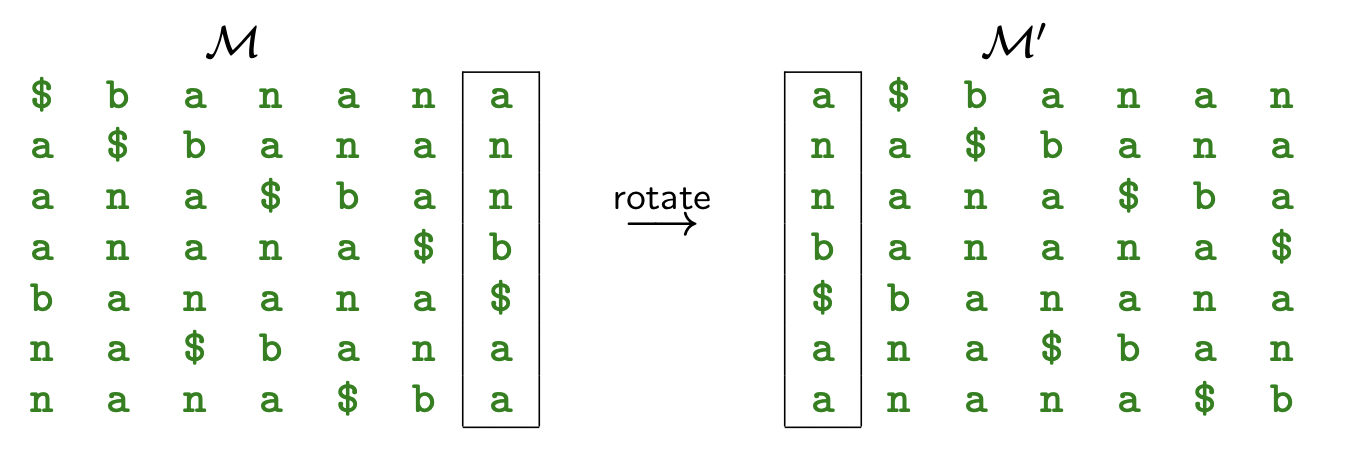
\includegraphics[width=1\textwidth]{Progetto Compressione Dati/capitoli/images/bwt.png}
\caption{Fonte: https://www.cs.helsinki.fi/u/tpkarkka/opetus/12k/dct/lecture08.pdf}
    \label{fig:bwt}
\end{figure}

\begin{figure}[h]
    \centering
    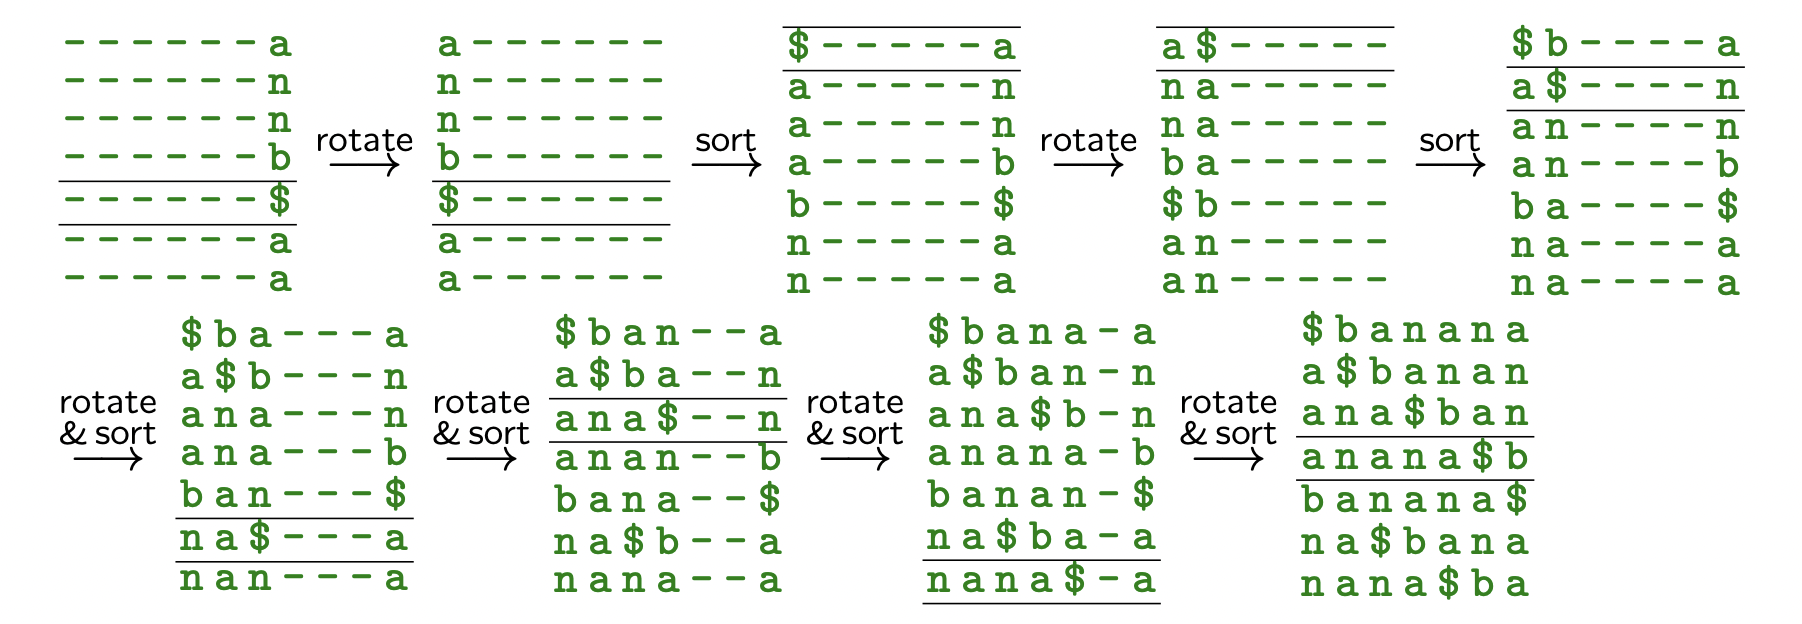
\includegraphics[width=1\textwidth]{Progetto Compressione Dati/capitoli/images/ibwt.png}
\caption{Fonte: https://www.cs.helsinki.fi/u/tpkarkka/opetus/12k/dct/lecture08.pdf}
    \label{fig:ibwt}
\end{figure}

Le figure \ref{fig:bwt} e \ref{fig:ibwt} chiariscono il funzionamento della trasformata e della sua inversa mediante un semplice esempio. 
\subsection{Move-to-Front} \label{section:mtf}
La \textbf{Move-to-Front (MTF)} è un algoritmo di codifica dei dati che consiste nel sostituire ogni simbolo della stringa input con la sua posizione in un alfabeto. Il funzionamento della \emph{MTF} si suddivide in tre step fondamentali:
\begin{enumerate}
    \item Data una stringa input $S$ definita su un alfabeto $\Sigma$, viene costruita una lista $L$ composta dai simboli di $\Sigma$ disposti secondo un certo ordinamento $K$;
    \item Per ogni simbolo $s$ di $S$ si codifica $s$ con la sua posizione $p$ in $L$, si aggiunge $p$ alla stringa $O$ da restituire in output e si sposta $s$ in cima alla lista $L$;
    \item L'output dell'algoritmo sarà la stringa $O$ e l'ordinamento $K$;
\end{enumerate}
Il vantaggio dell'utilizzo della \emph{MTF} risiede nel fatto che nel caso di input aventi lunghe sequenze di caratteri uguali, costruirà output aventi lunghe sequenze di $0$ in quanto i caratteri ripetuti avranno sempre la stessa posizione nell'alfabeto (che sarà proprio 0). La \emph{MTF} risulta essere invertibile a patto di conoscere l'ordinamento $K$ dei simboli dell'alfabeto $\Sigma$. Sostituendo, infatti, ogni simbolo della stringa codificata (che sarà un insieme di posizioni) con il carattere corrispondente nell'alfabeto $\Sigma$ al quale viene applicato l'ordinamento $O$ e portando tale carattere in cima all'alfabeto ad ogni iterazione, è possibile risalire alla stringa input. 
\begin{figure}[h]
    \centering
    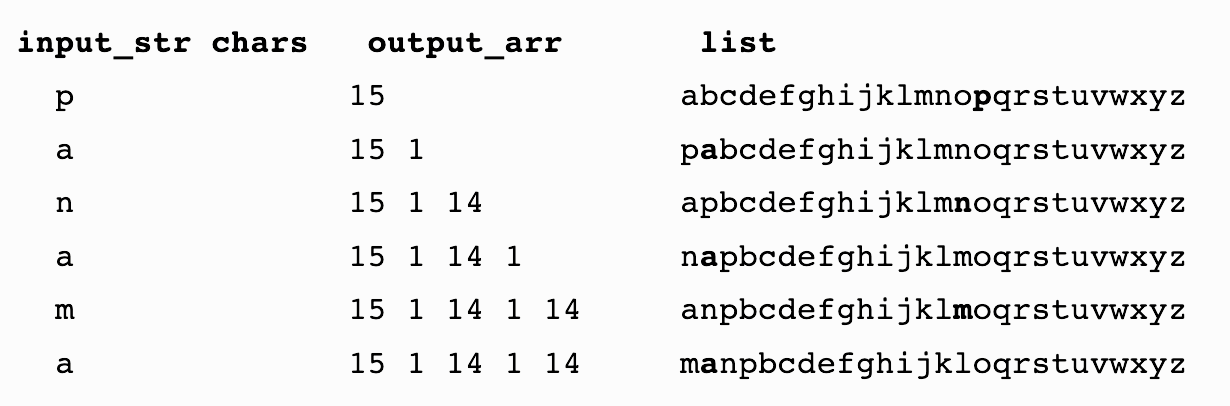
\includegraphics[scale=0.50]{Progetto Compressione Dati/capitoli/images/mtf.png}
\caption{Fonte: https://www.geeksforgeeks.org/move-front-data-transform-algorithm/}
    \label{fig:mtf}
\end{figure}
\begin{figure}[h]
    \centering
    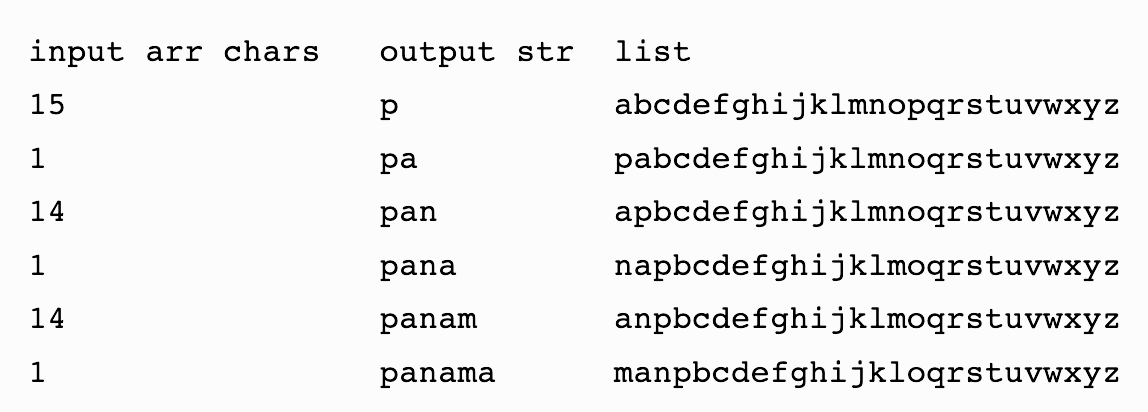
\includegraphics[scale=0.50]{Progetto Compressione Dati/capitoli/images/imtf.png}
\caption{Fonte: https://www.geeksforgeeks.org/inverting-move-front-transform/}
    \label{fig:imtf}
\end{figure} \\
Le figure \ref{fig:mtf} e \ref{fig:imtf} chiariscono il funzionamento della \emph{MTF} e della sua inversa mediante un semplice esempio. 

\subsection{Run-length encoding} \label{section:rle}
La \textbf{Run-length encoding} è il primo algoritmo di compressione che viene effettivamente utilizzato nella \emph{pipeline}. Tale algoritmo consiste nel rappresentare sequenze di caratteri ripetuti di una stringa in maniera compatta mediante l'utilizzo di un contatore, sostituendo le occorrenze multiple del carattere ripetuto in questione con una coppia $(c, counter)$, dove $c$ è il carattere ripetuto stesso e $counter$ indica il numero di volte in cui tale carattere si ripete. Tale algoritmo è banalmente invertibile sostituendo ogni coppia $(c, counter)$ con un numero di occorrenze di $c$ pari a $counter$. Il vantaggio dell'utilizzo della \emph{RLE} risiede nel fatto che, lavorando sull'output delle precedenti trasformate, si troverà a comprimere stringhe aventi lunghe sequenze consecutive di $0$. Tale caratteristica dell'input fa in modo che questo possa essere rappresentata in maniera concisa riducendone significativamente la lunghezza.  
\begin{figure}[h]
    \centering
    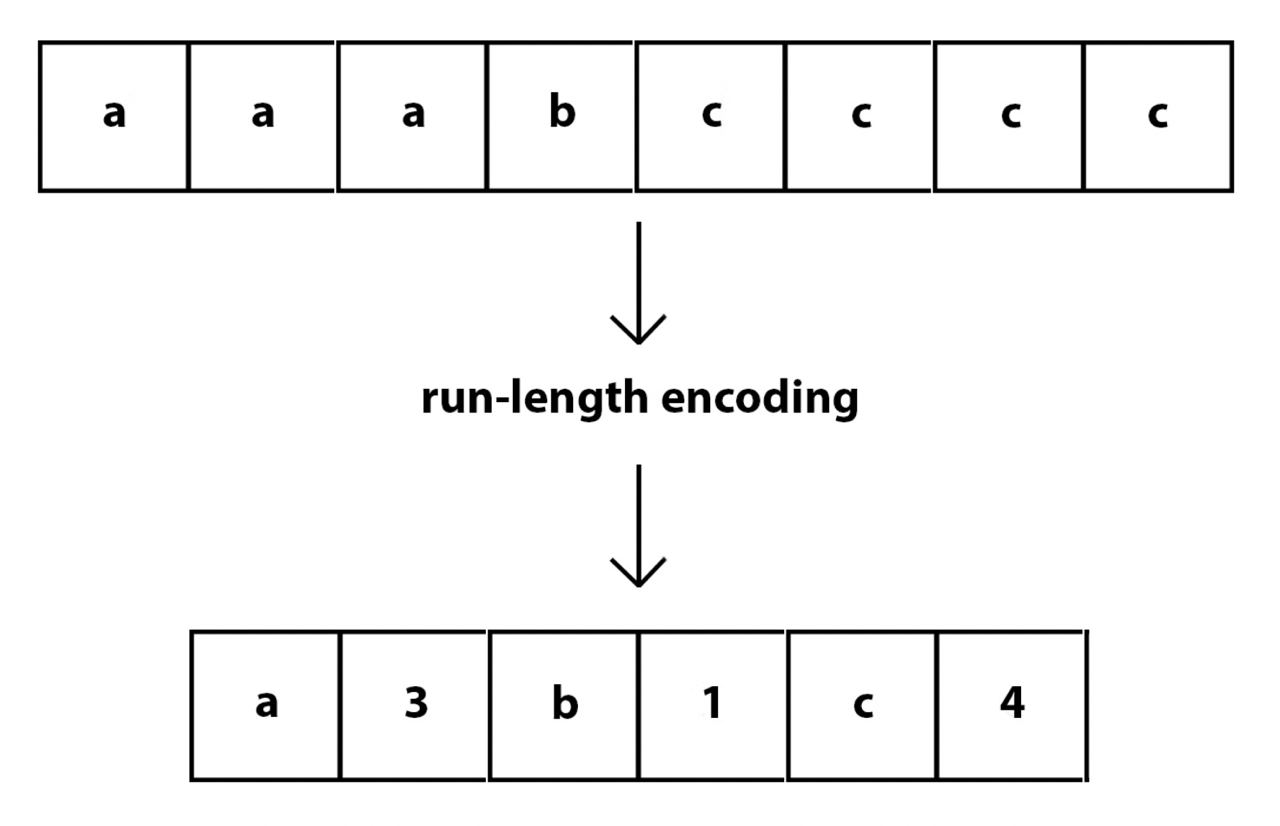
\includegraphics[width=0.5\textwidth, scale=0.5]{Progetto Compressione Dati/capitoli/images/rle.jpg}
\caption{Fonte: https://api.video/what-is/run-length-encoding}
    \label{fig:rle}
\end{figure} \\
La figura \ref{fig:rle} chiarisce il funzionamento della \emph{RLE} mediante un semplice esempio.
\subsection{Variable length Prefix Code} 
In generale, un algoritmo di \textbf{Variable length Prefix Code} consiste nel mappare i simboli della stringa sorgente su un numero variabile di bit. Alcune delle codifiche più note in letteratura sono \emph{Huffman coding}, \emph{Lempel-Ziv-Welch coding} e \emph{Arithmetic coding}. La scelta dell'algoritmo di \emph{Variable length Prefix Code} da inserire nella \emph{pipeline} influisce sul rapporto di compressione dell'algoritmo complessivo. Risulta opportuno sottolineare che tali algoritmi, essendo reversibili, possono essere utilizzati per la costruzione di un algoritmo di compressione \emph{lossless}.  
\section{Pipeline sicura}
La \emph{pipeline} presentata nel paragrafo precedente è strutturata in modo da far lavorare ogni algoritmo che la compone in sinergia con gli altri. Ciascun algoritmo descritto risulta, inoltre, facilmente invertibile, ragion per cui è possibile definire il processo di compressione complessivo \emph{lossless}. Ciò che manca a tale algoritmo è un layer di sicurezza, agevolmente implementabile negli algoritmi descritti mediante opportune modifiche che saranno trattate di seguito. Gli algoritmi interessati da tali modifiche sono la \emph{Burrows-Wheeler Transform} di cui verrà fornita la variante sicura denominata \emph{Scrambled Burrows-Wheeler Transform} e la \emph{Move-to-Front} di cui verrà fornita la versione sicura denominata \emph{Blocky Move-to-Front}. Il motivo per il quale è necessario distribuire il layer di sicurezza su due algoritmi risiede nel fatto che precedenti tentativi da parte di ricercatori di costruire un algoritmo modificando unicamente la \emph{BWT} hanno "scoperto il fianco" ad attacchi di tipo statistico \cite{stanek2012attacking}. Attuando opportune modifiche alla \emph{MTF} è possibile rendere l'algoritmo di compressione complessivo sicuro rispetto a tali attacchi. L'algoritmo di compressione \emph{lossless} sicuro prenderà in input un testo $T$ da comprimere e una chiave segreta $K$ e sarà composto da \emph{Scrambled Burrows-Wheeler Transform, Blocky Move-To-Front, Run-Length Encoding e Variable Length Prefix Code}, restituendo un testo compresso $C$. Specularmente, l'algoritmo di decompressione prenderà in input il testo compresso $C$ e la chiave segreta $K$ e sarà composto da \emph{Inverse Variable Length Prefix Code, Inverse Run-Length Encoding, Inverse Blocky Move-To-Front e Inverse Scrambled Burrows-Wheeler Transform}, restituendo il testo non compresso di partenza $T$. La sicurezza della \emph{pipeline} appena descritta poggia le proprie fondamenta sul concetto di \textbf{IND-CPA sicurezza}. Intuitivamente, tale nozione di sicurezza garantisce che un avversario a cui non è nota la chiave segreta $K$ non sia in grado di stabilire se un testo compresso $C$ sia il risultato della compressione sicura di una stringa $T_0$ o di una stringa $T_1$ (dove $T_0$ e $T_1$ sono stringhe \emph{isomorfe}\footnote{Due stringhe $s$ e $t$ sono isomorfe se ogni occorrenza di ogni carattere di $s$ può essere sostituita per ottenere $t$ mantenendo l'ordinamento dei caratteri, e.g., \emph{egg} e \emph{add} sono stringhe isomorfe, mentre \emph{foo} e \emph{bar} non lo sono.} scelte dall'avversario stesso che ha accesso ad un oracolo di compressione che comprime utilizzando $K$) sfruttando una strategia migliore del "tirare a indovinare". Gli autori di \cite{zeng2018secure} forniscono, oltre che una definizione formale di \emph{IND-CPA sicurezza}, una prova del fatto che l'algoritmo in questione sia \emph{IND-CPA sicuro}. Nei prossimi paragrafi verranno descritte le modifiche da apportare agli algoritmi per far sì che l'algoritmo di compressione soddisfi tale nozione di sicurezza. 
\subsection{Scrambled Burrows-Wheeler Transform} \label{section:sbwt}
Per aggiungere un layer di sicurezza alla \emph{BWT} è possibile modificarla in modo tale che questa prenda in input una chiave segreta $K$, mediante la quale viene calcolato un ordinamento lessicografico segreto che servirà per disporre le righe della matrice generata dall'algoritmo. L'algoritmo risultante da tale modifica, denominato \textbf{Scrambled Burrows-Wheeler Transform} prende in input:
\begin{itemize}
    \item una stringa $S$ da comprimere definita su un alfabeto $\Sigma$;
    \item una chiave segreta $K$;
    \item una funzione di permutazione basata su chiave $Perm$;
\end{itemize}
Il funzionamento dell'algoritmo si suddivide in quattro step fondamentali:
\begin{enumerate}
    \item Si sceglie un numero random $r$ e si computa $Perm(r, K)\rightarrow\xi$, dove $\xi$ denota l'ordinamento lessicografico segreto;
    \item Si aggiunge un carattere speciale $\$ \notin \Sigma$ alla fine della stringa $S$ ottenendo la stringa $S'$. Il carattere $\$$ sarà più piccolo in ordine lessicografico rispetto ad ogni altro carattere di $\Sigma$;
    \item Si costruisce una matrice $M$ le cui righe sono gli shift ciclici di $S'$;
    \item Si dispongono le righe di $M$ nell'ordine lessicografico segreto $\xi$ ottenendo la matrice $M'$ e si restituisce l'ultima colonna di $M'$ come risultato della \emph{sBWT};
\end{enumerate}
L'unica differenza tra le due versioni dell'algoritmo risiede nel fatto che mentre nella \emph{BWT} le righe della matrice $M$ vengono disposte in ordine lessicografico, nella \emph{sBWT} tale ordinamento lessicografico varia in base alla chiave $K$. L'utilizzo di un ordinamento lessicografico fa sì che anche le stringhe di output della \emph{sBWT} presentino lunghe sequenze di caratteri ripetuti, dunque il vantaggio intrinseco della \emph{BWT} viene preservato anche nella sua versione sicura. La proprietà di invertibilità della \emph{sBWT} vale a patto di conoscere l'ordinamento lessicografico segreto utilizzato per disporre le righe della matrice $M$. In altri termini è necessario conoscere la chiave segreta $K$, il numero random $r$ generato in fase di compressione e la funzione di permutazione $Perm$. \\
\subsection{Blocky Move-to-front} {\setstretch{1.3}
La modifica da apportare alla \emph{Move-to-front} al fine di aggiungere un layer di sicurezza non differisce molto da quella che interessa la \emph{BWT}. Anche questa revisione dell'algoritmo, infatti, poggia la proprie fondamenta sulla costruzione di permutazioni segrete dell'alfabeto utilizzato. In particolare, la versione sicura della \emph{MTF}, denominata \textbf{Blocky Move-to-front} prende in input: 
\begin{itemize}
    \item una stringa $S$ da comprimere definita su un alfabeto $\Sigma$;
    \item un parametro intero $L$ che indica la dimensione del blocco;
    \item una chiave segreta $K$;
    \item una funzione di permutazione basata su chiave $Perm$;
    \item un vettore di inizializzazione $IV$;
    \item una funzione hash $f$
\end{itemize}
Il funzionamento dell'algoritmo si suddivide in tre step fondamentali:
\begin{enumerate}
    \item La stringa $S$ viene suddivisa in un certo numero di blocchi, ciascuno dei quali costituito da $L$ caratteri;
    \item Per ogni blocco $block_i$ si costruisce una permutazione $Perm(K, IV$ or $f(block_{i-1})) \rightarrow \xi_i$ dei caratteri nell'alfabeto $\Sigma$. Durante la prima iterazione dell'algoritmo il secondo parametro di $Perm$ è $IV$, mentre durante le iterazioni successive sarà l'hash (calcolato mediante la funzione $f$) del blocco precedente;
    \item Per ogni blocco $block_i$ costruito si eseguono gli step classici della $MTF$ utilizzando l'ordinamento segreto computato;
\end{enumerate}
Nel momento in cui la \emph{bMTF} si trova a lavorare sugli output della \emph{sBWT} produce stringhe contenenti lunghe sequenze di $0$. La lunghezza di tali sequenze dipende dal valore del parametro $L$: più grande sarà questo parametro, più lunga sarà la sequenza. Una trattazione relativa alla scelta del parametro $L$ verrà svolta nei capitoli successivi. Dal momento che la \emph{bMTF} lavora permutando l'alfabeto ogni $L$ caratteri non è possibile per un avversario condurre attacchi di tipo statistico come accadeva nel caso in cui l'unico algoritmo della \emph{pipeline} interessato dalle revisioni di sicurezza era la \emph{BWT}. L'invertibilità della \emph{bMTF} è garantita a patto di conoscere le permutazioni corrispondenti ad ogni blocco dell'input. In altri termini è necessario conoscere la chiave segreta $K$, il vettore di inizializzazione $IV$, la dimensione del blocco $L$, la funzione di permutazione $Perm$ e la funzione hash $f$. 
}